\documentclass[12 pt,letterpaper]{article}
\usepackage[spanish]{babel}
\usepackage[utf8]{inputenc}
\usepackage{amsmath}
\usepackage{amssymb}
\usepackage{ragged2e}
\usepackage{xspace}
\usepackage{graphicx}
\usepackage{graphics}
\usepackage{amsmath}
\usepackage{csquotes}
\usepackage{float}
\usepackage{url}
\usepackage{listings}
\usepackage{biblatex}
\usepackage{xcolor}
\newcommand{\bibTitle}[1]{``#1''}
\usepackage{geometry}
\geometry{left=3cm,right=2cm,top=2cm,bottom=2cm}
\author{Marisol Chacua Cuaspa}
\usepackage{listings}
\lstset{literate=
  {á}{{\'a}}1 {é}{{\'e}}1 {í}{{\'i}}1 {ó}{{\'o}}1 {ú}{{\'u}}1
  {Á}{{\'A}}1 {É}{{\'E}}1 {Í}{{\'I}}1 {Ó}{{\'O}}1 {Ú}{{\'U}}1
  {à}{{\`a}}1 {è}{{\`e}}1 {ì}{{\`i}}1 {ò}{{\`o}}1 {ù}{{\`u}}1
  {À}{{\`A}}1 {È}{{\'E}}1 {Ì}{{\`I}}1 {Ò}{{\`O}}1 {Ù}{{\`U}}1
  {ä}{{\"a}}1 {ë}{{\"e}}1 {ï}{{\"i}}1 {ö}{{\"o}}1 {ü}{{\"u}}1
  {Ä}{{\"A}}1 {Ë}{{\"E}}1 {Ï}{{\"I}}1 {Ö}{{\"O}}1 {Ü}{{\"U}}1
  {â}{{\^a}}1 {ê}{{\^e}}1 {î}{{\^i}}1 {ô}{{\^o}}1 {û}{{\^u}}1
  {Â}{{\^A}}1 {Ê}{{\^E}}1 {Î}{{\^I}}1 {Ô}{{\^O}}1 {Û}{{\^U}}1
  {ã}{{\~a}}1 {ẽ}{{\~e}}1 {ĩ}{{\~i}}1 {õ}{{\~o}}1 {ũ}{{\~u}}1
  {Ã}{{\~A}}1 {Ẽ}{{\~E}}1 {Ĩ}{{\~I}}1 {Õ}{{\~O}}1 {Ũ}{{\~U}}1
  {œ}{{\oe}}1 {Œ}{{\OE}}1 {æ}{{\ae}}1 {Æ}{{\AE}}1 {ß}{{\ss}}1
  {ű}{{\H{u}}}1 {Ű}{{\H{U}}}1 {ő}{{\H{o}}}1 {Ő}{{\H{O}}}1
  {ç}{{\c c}}1 {Ç}{{\c C}}1 {ø}{{\o}}1 {å}{{\r a}}1 {Å}{{\r A}}1
  {€}{{\euro}}1 {£}{{\pounds}}1 {«}{{\guillemotleft}}1
  {»}{{\guillemotright}}1 {ñ}{{\~n}}1 {Ñ}{{\~N}}1 {¿}{{?`}}1 {¡}{{!`}}1 
}

\begin{document}
	
	
	\begin{titlepage}
		\centering
		
		\vspace{1cm}
		{\bfseries\LARGE Universidad del Cauca \par}
		\vspace{5cm}
		
		{\scshape\Large Campos de direcci\'on y el m\'etodo de aproximaci\'on de Euler y Euler mejorado\par}
		\vspace{3cm}
		{\Large Curso de verano: Ecuaciones Diferenciales\par}
		\vfill
		{\Large Marisol Chacua Cuaspa \par}
		\vfill
		{\Large Jhonatan Collazos Ramírez \par}
		\vfill
        {\Large Facultad de ingenieria civil\par}
		{\Large Popayán\par}
	    {\Large Agosto 2022\par}
	\end{titlepage}
	
	\centering
	\textbf{\LARGE{INTRODUCCI\'ON }}
	
	
	\justify 
   En ingeniería hemos aprendido diferentes métodos matemáticos para resolver sistemas de ecuaciones, integrales, gráficas, etc. En el ámbito de ecuaciones diferenciales ordinarias, se emplean varios procedimiento para evaluar el comportamiento de las soluciones. La ecuación diferencial nos indica que la pendiente de una curva solución en un punto {$(x, y)$} sobre la curva es:{$ f(x, y)$}  . Si se dibujan segmentos de recta cortos con pendientes {$ f(x, y)$} en varios puntos  {$x, y$}, el resultado se llama campo direccional (campo de pendientes). Visualmente, la dirección del campo indica el aspecto o forma de una familia de curvas solución de la ecuación diferencial dada y, en consecuencia, se pueden ver a simple vista aspectos cualitativos de la solución.Una técnica útil para visualizar (graficar) las soluciones de una ecuación diferencial de primer orden consiste en bosquejar el campo de direcciones de la ecuación. Para describir este método, necesitamos una observación general:{\itshape\ Una ecuación de primer orden.}\vspace{0.4Cm}
 
	El método de Euler es el más básico y sencillo de los procedimientos usados para encontrar soluciones numéricas aproximadas, a una ecuación diferencial ordinaria de primer orden, siempre que se conozca su condición inicial. La idea del método de Euler es encontrar una solución numérica a la ecuación diferencial en el intervalo comprendido entre {$x_{0} $} y {$x_{f} $} .	\vspace{0.4Cm}

	El método de Euler mejorado consiste en tomar las fórmulas del método de Euler para calcular la pendiente en un punto inicial y en un punto final y luego promediarlas. De esta manera el resultado será mucho más acertado a lo largo de todo el intervalo.\vspace{0.4Cm}
	
	Es importante resaltar que estos métodos no pretenden encontrar la forma concreta de la función que da solución a la ecuación diferencial, sino sus valores ya que estos son los que realmente importan.\vspace{0.4Cm}
\newpage
	
	
	\flushleft\section{\fbox{\textcolor{violet}{Aplicaciones}}}
	
	
	\flushleft\subsection{\underline{Campos de dirección}}\vspace{0.5cm}
	
	
	\begin{enumerate}
	\justify
    Campos de direcciones (también llamados campos de pendiente) son útiles para investigar las ecuaciones diferenciales de primer orden. En particular, consideramos una ecuación diferencial de primer orden de la forma\[y'=f(x,y)\]Un ejemplo aplicado de este tipo de ecuación diferencial aparece en la ley de enfriamiento de Newton.La idea de un campo de direcciones es el hecho de que la derivada de una función evaluada en un punto determinado es la pendiente de la línea tangente al gráfico de esa función en el mismo punto. Podemos utilizar un campo de direcciones para predecir el comportamiento de las soluciones de una ecuación diferencial sin conocer la solución real. \bibTitle{1}
		
	\end{enumerate} 
	
	
	\flushleft\subsection{\underline{Aproximación de Euler}}\vspace{0.5cm}
	
   \begin{itemize}
   \item\justify 
   El método de Euler rara vez se utiliza en la práctica para obtener la solución aproximada de un problema de valor inicial, pero se estudia por su simplicidad en la derivación de la fórmula y de la determinación del error. Los métodos de orden superior utilizan las mismas técnicas, pero el álgebra que requieren es mucho más complicada. Con el método de Euler se obtiene una solución aproximada de un problema de valor inicial, en un conjunto finito de puntos.El método de Euler (o método de la recta tangente) es un procedimiento que permite construir aproximaciones a las soluciones de un problema con valor inicial, para una ecuación diferencial ordinaria de primer orden.

   \begin{flushleft}
\fbox{\textcolor{purple}{Ejercicio de aplicación}}\vspace{0.5cm}
	\end{flushleft}

	\justify 
    Consideremos el problema de calcular la forma de una curva desconocida que comienza en un punto determinado y satisface una ecuación diferencial dada. En este caso, una ecuación diferencial puede considerarse como una fórmula mediante la cual se puede calcular la pendiente de la recta tangente a la curva en cualquier punto de la misma, una vez que se ha calculado la posición de ese punto. La idea es que mientras la curva es inicialmente desconocida, su punto de partida, que denotamos por {$A_{0} $}, es conocido. Entonces, a partir de la ecuación diferencial, se puede calcular la pendiente de la curva en {$A_{0} $} y, por tanto, la línea tangente.
			
	Demos un pequeño paso a lo largo de esa línea tangente hasta un punto {$A_{1} $}. A lo largo de este pequeño paso, la pendiente no cambia demasiado, por lo que {$A_{1} $} estará cerca de la curva. Si pretendemos que {$A_{1} $} sigue en la curva, se puede utilizar el mismo razonamiento que para el punto {$A_{0} $} anterior. Después de varios pasos, se calcula una curva poligonal {$A_{0} $}, {$A_{1} $}, {$A_{2} $}, {$A_{3} $}.... En general, esta curva no diverge demasiado de la curva original desconocida, y el error entre las dos curvas puede hacerse pequeño si el tamaño del paso es suficientemente pequeño y el intervalo de cálculo es finito: \[y'(t)= f(t,y(t)), \hspace{1cm}  y'(t_{0}=y_{0}) \]\vspace{0.3cm}

        Elegir un valor h para el tamaño de cada paso y establecer
		\[ 
		t_{n}=t_{0}+nh
		\]
		\vspace{0.5cm}
		Ahora, un paso del método de Euler desde $t_{n}$ hasta $t_{n+1} = t_{n+h}$ es:
		\[ 
		(y_{n+1}=y_{n}+hf(t_{n},y_{n}))
		\]
		\vspace{0.5cm}
		El valor de  \[y_{n}\]  es una aproximación a la solución de la EDO en el tiempo \[y_{n}\approx y(t_{n})\]
        
 	
	\end{itemize}

\flushleft\subsubsection{\underline{\textit{Ejercicio 1: Metodo de aproximación de Euler}}}\vspace{0.5cm}

   \begin{itemize}
       \item Dada el PVI\hspace{1cm} \textbf{Y’=2x-3y+1}
       \item y(1)=5 \hspace{2cm} h=0.05
       \item Aproximar y(1.2)
   \end{itemize}\leavevmode\newline

    Solución:
    \begin{equation}
    \frac{dy}{dx}=f(x,y)
    \end{equation}
\begin{equation}
    \frac{dy}{dx}=2x-3y+1
    \end{equation}
$x_{0}=1$\\
$y_{0}=5$\\
$h=0.05$\\
\vspace{4mm} %5mm vertical space
Desarrollamos hasta el valor buscado en x, en este caso \textbf {x=1,2}\\
\vspace{4mm} %5mm vertical space
\begin{itemize}
\item\textbf{$y_{0}+1=y_{0}+h(f(x_{0},y_{0}))$}\\
\item\textbf{$x_{1}=x_{0}+h  \Rightarrow x_{1}=1+0.05\Rightarrow x_{1}=1.05 $} \\
{$y_{1}=y_{0}+h(2x_{0}-3y_{0}+1))$}\\
{$y_{1}=5+(0.05)(2(1)-3(5)+1))$}\\
{$y_{1}=5+(0.05)(2-15+1))$}\\
{$y_{1}=5-0.6$}\\
{$y_{1}=4.4$}\\
\textbf{$y_{(1.05)}=4.4$}\\
\end{itemize}
\vspace{0.8mm} %5mm vertical space
\begin{itemize}
\item\textbf{$x_{2}=x_{1}+h  \Rightarrow x_{2}=1.05+0.05\Rightarrow x_{2}=1.1 $} \\
\item\textbf{$y_{2}=y_{1}+h(2x_{1}-3y_{1}+1))$}\\
{$y_{2}=4.4+(0.05)(2(1.05)-3(4.4)+1))$}\\
{$y_{2}=4.4+(0.05)(-10.1)$}\\
{$y_{2}=4.4-(0.505)$}\\
{$y_{2}=3.89$}\\
\textbf{$y_{(1.1)}=3.89$}\\
\end{itemize}
\vspace{0.5mm} %5mm vertical space
\begin{itemize}
\item\textbf{$x_{3}=x_{2}+h  \Rightarrow x_{3}=1.1+0.05\Rightarrow x_{3}=1.15 $} \\
\item\textbf{$y_{3}=y_{2}+h(2x_{2}-3y_{2}+1))$}\\
{$y_{3}=3.89+(0.05)(2(1.1)-3(3.89)+1))$}\\
{$y_{3}=3.89+(0.05)(-8.47)$}\\
{$y_{3}=3.89-(0.42)$}\\
{$y_{3}=3.47$}\\
\textbf{$y_{(1.15)}=3.47$}\\
\end{itemize}
\vspace{0.5mm} %5mm vertical space
\begin{itemize}
\item\textbf{$x_{4}=x_{3}+h  \Rightarrow x_{4}=1.15+0.05\Rightarrow x_{4}=1.2 $} \\
\item\textbf{$y_{4}=y_{3}+h(2x_{3}-3y_{3}+1))$}\\
{$y_{4}=3.47+(0.05)(2(1.15)-3(3.47)+1))$}\\
{$y_{4}=3.47+(0.05)(-7.11)$}\\
{$y_{4}=3.47-(0.35)$}\\
{$y_{4}=3.12$}\\
\textbf{$y_{(1.2)}=3.12$}\\
\end{itemize}
En el cuadro 1. se puede observar los valores desde {$x=1$} hasta {x=1.2 }en pasos de 0.05, obtenierno asi los valores de la funcion que se representan en la columna  y.\\
\begin{table}[H]
\centering
\begin{tabular}{|c|c|c|}
   \hline
interacción & x & y\\
\hline
 & 1 & 5\\
\hline
1 & 1,05 & 4,4\\
\hline
2& 1,1 & 3,89\\
\hline
3& 1,15 & 3,47\\
\hline
4& 1,2 & 3,12\\
\hline
\end{tabular}
\caption{Aproximación a la solución de la EDO \\}

\end{table}

A continuación se encuentra el código empleado en mathlab, con el cual es posible resolver la ecuación anteriomente mensionada como ejercicio.
\begin{lstlisting}
%Ejercicio 1:Método de aproximación  de Euler
clear all;
close all;
clc;

syms x y
f(x,y)=input('Enter function in form of dy/dx=f(x,y):');

%Valores iniciales
i=1;
x0(i)=input('Enter x0=');
y0(i)=input('Enter y0=');

xn=input('Enter upper limit of interval xn='); %Alcance de la grafica de aproximacion 
h=input('Enter width (equal space) h='); %Incremento
n=(xn-x0)/h; %Numero de iteraciones

xapro=input('Enter value to aproximate=');%Numero a aproximar

fprintf('--------------------------------------------\n')
fprintf('    xi            yi           \n');
fprintf('--------------------------------------------\n')

for i=1:(n+1)
    
    y1(i)=y0(i)+h*subs(subs(f,x,x0(i)),y,y0(i));
    x0(i+1)=x0(i)+h;
    y2(i)=y0(i)+h*(subs(subs(f,x,x0(i)),y,y0(i)) + subs(subs(f,x,x0(i+1)),y,y1(i)))/2;
    fprintf('%f      %f       \n',x0(i),y0(i))
    y0(i+1)=y2(i);
    
end

plot(x0,y0,'*-');grid on;

%Solucion real
syms y(x)
dy = diff(y(x),x);
Y(x) = dsolve(dy== f(x,y), y(x0(1))==y0(1)); %Sol. real de la ED
fprintf('\n')
fprintf('Solución real:\n')
disp(Y(x))
hold on;
fplot(Y(x),'+-',[-1 2])

title('Aproximacion vs Solucion analítica')
legend('aprox.','sol. real')

%Error absoluto
Er = Y(xapro) - y0(round((xapro-x0(1))/h+1));

%Mostrando resultados
fprintf('La solución aproximada evaluada en x=%f es: %f',xapro ,y0(round((xapro-x0(1))/h+1)))
fprintf('\n\n')
fprintf('La solución real evaluada en x=%f es: %f',xapro,Y(xapro))
fprintf('\n\n')
fprintf('Error absoluto: %f', Er)
	\end{lstlisting}
	
	\flushleft\subsection{\underline{Euler Mejorado}}\vspace{0.5cm}
	
	\begin{itemize}
 \item\justify 
    En la historia de las matemáticas, siempre han estado presentes los métodos de soluciones aproximadas, desde soluciones de funciones polinomiales, hasta problemas de astronomía, este método  ha sido parte importante en el desarrollo de la ciencia y de la ingeniería. Uno de los métodos más antiguos que dan soluciones aproximadas a las ecuaciones diferenciales es el método de Euler.
    Se utiliza el método de Euler Mejorado para discretizar la variable espacial de la ecuación de transporte de neutrones, éste método es un técnica numérica de primer orden, que da solución a las ecuaciones diferenciales ordinarias, utilizando un valor inicial conocido. Para disminuir el error, el método utiliza un valor promedio de la derivada, tomada en los dos extremos del intervalo, en lugar de la derivada tomada en un solo extremo, definido por la fórmula:
.
    

	\begin{equation}
   y_{n+1}=y_{n}+h\frac{f(x_{n},y_{n})+f(x_{n+1},y^*_{n+1})}{2}
    \end{equation}

donde

 
	\begin{equation}
   y^*_{n+1}=y_{n}+hf(x_{n},y_{n})
    \end{equation}\vspace{0.3Cm}

Para cálcular $y_{n+1}$ para $n=0,1,2...$ de (1),se debe en cada paso, usar primero el método de Euler(2) para tener una estimación inicial $y^*_{n+1}$. Por ejemplo, con $n=0$, usando (2) se obtiene  $y^*_{n}= y_{n}+hf(x_{0},y_{0})$, y después, conociendo este valor, se usa (1) para obtener  $y_{n+1}=y_{n}+h\frac{f(x_{n},y_{n})+f(x_{n+1},y^*_{n+1})}{2}$, donde $x_{1}=x_{0}+h$. Estas ecuaciones se representan con facilidad.

\begin{figure}[H]
    \centering
    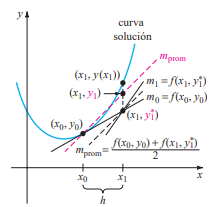
\includegraphics{Pendiente de la recta roja.png}
    \caption{pendiente de la recta roja
punteada esel promedio de $m_{0}$ y $m_{1}$}
    \label{pendiente}
\end{figure}\vspace{0.2Cm}
 \begin{flushleft} 
En la Figura \ref{pendiente} se observa $m_{0}=f(x_{0},y_{0})$  y $m_{1}=f(x_{1},y_{1})$ son pendientes de las rectas trazadas con la línea continua que pasan por los puntos $(x_{0},y_{0})$  y  $(x_{1},y^*_{1})$, respectivamente. Tomando un promedio de estas pendientes, es decir, $m_{prom} =\frac{f(x_{n},y_{n})+f(x_{n+1},y^*_{n+1})}{2}$, se obtiene la pendiente de las rectas paralelas inclinadas.
Con el primer paso, más que avanzar a lo largo de la recta que pasa por $(x_{0},y_{0})$  con pendiente $f(x_{0},y_{0})$  al punto de coordenada y $y^*_{1}$  obtenida por el metodo de Euler, se avanza a lo largo de la recta punteada de color rojo que pasa por $(x_{0},y_{0})$  con pendiente $m_{prom}$  hasta llegar a $x_{1}$.Al examinar la figura parece posible que  $y_{1}$ sea una mejora de  $y^*_{1}$.\\
En general, el método de Euler mejorado es un ejemplo de un \textbf{método de predicción-corrección}. El valor de $y^*_{n+1}$ dado por (2) predice un valor $y(x_{n})$, mientras que el valor de $y_{n+1}$ definido por la fómula (1) corrige esta estimación.\\
\end{flushleft} 
\begin{flushleft}
\fbox{\textcolor{purple}{Ejercicio de aplicación}}\vspace{0.cm}
\end{flushleft}

\flushleft\subsubsection{\underline{\textit{Ejercicio 2: Método de Euler mejorador}}}\vspace{0.5cm}
\begin{flushleft}
\item\justify
Use el metodo de Euler mejorado para obtener el valor aproximado de $y(1.5)$ para la solución del problema con valores iniciales $ y'$ $= 2xy,  y(1) = 1$. Obtener resultados para $h = 0.1 $
\item\justify{\textbf{Solución}}\\
Para obtener el valor real solucionamos la ecuacion diferencial, la cual es de variable separable:
\end{flushleft}
\begin{flushleft}
  \begin{equation}
    \frac{dy}{dx}=2xy
    \end{equation}
\begin{equation}
    \frac{dy}{y}=2x dx
    \end{equation}
\begin{equation}
\int{\frac{dy}{y}=\int{2x dx}}
\end{equation}

\[ln(y) = x^{2}+ C\]\\
\[e^{ln(y)} = e^{x^{2}+c}\]
\[y = k*e^{x^2}\]
sustituyendo el valor inicial queda\\
\[y = e^{x^2-1}\]
Luego, haciendo uso del método de Euler Mejorado se procede a resolver de la sigueinte manera:\\
$x_{0}=1$\\
$y_{0}=1$\\
$h=0.1$\\
Primero se calcula el valor de la ecuación (4)
\vspace{0.5mm} %5mm vertical space
\begin{flushleft}
 \begin{center}
   $y^*_{1}=y_{0}+(0.1)(2x_{0},y_{0})=1+(0.1)(2(1)(1))=1.2$
    \end{center}
\end{flushleft}\vspace{0.1Cm}
se usa este ultimo valor en (3) junto con $ x_{1}=1+h=1+0.1=1.1$
\begin{flushleft}
$y_{1}=y_{0}+(0.1) \frac{2x_{0},y_{0}+2x_{1},y^*_{1}}{2}=1+(0.1) \frac{2(1)(1)+2(1.1)(1.2)}{2}=1.232$
\end{flushleft}

sustituyendo en las fórmulas, los calculos para $h=0.1$ seran representados en el siguiente cuadro :\\
\end{flushleft}
\begin{table}[H]
\centering
\begin{tabular}{|c|c|c|c|c|}
   \hline
 $x_{n}$& $y_{n}$ & Valor real&valor absoluto& porcentaje relativo\\
\hline
 $1.00$& $1.0000$ &$1.0000$& $0.0000$& $0.00$\\
$1.10$& $1.2320$& $1.2337$&$ 0.0017$& $0.14$\\
$1.20 $&$1.5479$&$ 1.5527 $&$0.0048$&$ 0.31$\\
$1.30$&$ 1.9832$&$ 1.9937$&$ 0.0106$&$ 0.53$\\
$1.40$&$ 2.5908$&$ 2.6117$&$ 0.0209 $&$0.80$\\
$1.50 $&$3.4509$&$ 3.4904$&$ 0.0394$&$ 1.13$\\
\hline
\end{tabular}
 \caption{Método de Euler Mejorado con $h=0.1$}
    \label{}
\end{table}
La  solución de la anterior ecuación  fue comprobada con el programa Mathlab en en cual se utilizo el siguiente código para dicha ejecución.
	\begin{lstlisting}
	% Numerical Method 
% Improved Euler method using MATLAB 

%%Nota1: La n tiene que dar un numero entero. Mientras la h sea mas pequeña
%%es mas probable que la n sea entera.

%%Nota2: Si vas a resolver una ecuacion que no tiene solucion analitica el
%%program te va a lanzar error, tendras que borrar la seccion de la solucion real y lo que
%%tenga asociado.

clear all;
close all;
clc;

syms x y
f(x,y)=input('Enter function in form of dy/dx=f(x,y):');

%Valores iniciales
i=1;
x0(i)=input('Enter x0=');
y0(i)=input('Enter y0=');

xn=input('Enter upper limit of interval xn='); %%Alcance de la
%%grafica de aproximacion 
h=input('Enter width (equal space) h='); %Incremento
n=(xn-x0)/h; %Numero de iteraciones

xapro=input('Enter value to aproximate=');%Numero a aproximar

fprintf('--------------------------------------------\n')
fprintf('    xi            yi           \n');
fprintf('--------------------------------------------\n')

for i=1:(n+1)
    
    y1(i)=y0(i)+h*subs(subs(f,x,x0(i)),y,y0(i));
    x0(i+1)=x0(i)+h;
    y2(i)=y0(i)+h*(subs(subs(f,x,x0(i)),y,y0(i)) + subs(subs(f,x,x0(i+1)),y,y1(i)))/2;
    fprintf('%f      %f       \n',x0(i),y0(i))
    y0(i+1)=y2(i);
    
end

plot(x0,y0,'*-');grid on;

%Solucion real
syms y(x)
dy = diff(y(x),x);
Y(x) = dsolve(dy== f(x,y), y(x0(1))==y0(1)); %Sol. real de la ED
fprintf('\n')
fprintf('Solución real:\n')
disp(Y(x))
hold on;
fplot(Y(x),'+-',[-1 2])
title('Aproximacion vs Solucion analítica')
legend('aprox.','sol. real')

%Error absoluto
Er = Y(xapro) - y0(round((xapro-x0(1))/h+1));

%Mostrando resultados
fprintf('La solución aproximada evaluada en x=%f es: %f',xapro ,y0(round((xapro-x0(1))/h+1)))
fprintf('\n\n')
fprintf('La solución real evaluada en x=%f es: %f',xapro,Y(xapro))
fprintf('\n\n')
fprintf('Error absoluto: %f', Er)
	\end{lstlisting}
	\newpage
\begin{thebibliography}{99}
\small

\bibitem {1} {NAGLE, R. Kent; SAFF, Edward B.; SNIDER, Arthur David. Ecuaciones diferenciales y problemas con valores en la frontera. Pearson Educación, 2000..Pág:16} 

\bibitem {2} {NAGLE, R. Kent; SAFF, Edward B.; SNIDER, Arthur David. Ecuaciones diferenciales y problemas con valores en la frontera. Pearson Educación, 2000..Pág:24} 

\bibitem {3} {NAGLE, R. Kent; SAFF, Edward B.; SNIDER, Arthur David. Ecuaciones diferenciales y problemas con valores en la frontera. Pearson Educación, 2000.Pág:340} 

\bibitem {4} {ZILL, Dennis G.; HERNÁNDEZ, Ana Elizabeth García; LÓPEZ, Ernesto Filio. Ecuaciones diferenciales con aplicaciones de modelado. Thomson Learning, 2002.} 

\bibitem {1} {Ejercicio aproximación de Euler} 
\bibTitle{Aproximacion de euler}, 
\url{https://en.wikipedia.org/wiki/Euler_method#:~:text=The%20Euler%20method%20is%20a,proportional%20to%20the%20step%20size./},

\bibitem {1} {Ejercicio de Euler mejorado} 
\bibTitle{NAGLE, R. Kent; SAFF, Edward B.; SNIDER, Arthur David. Ecuaciones diferenciales y problemas con valores en la frontera. Pearson Educación, 2000..Pág:343},










\end{thebibliography}

	\end{itemize}
\end{document}











